\documentclass[a4paper,12pt]{article}
%%%%%%%%%%%%%%%%%%%%%%%%%%%%%%%%%%%%%%%%%%%%%%%%%%%%%%%%%%%%%%%%%%%%%%%%%%%%%%%%%%%%%%%%%%%%%%%%%%                  PREAMBULO
%
%a4paper = 21cm por 29,7cm; 1in= 2,54cm; 1cm= 28pt
%
%
\usepackage{amssymb}
\usepackage{amsmath}
\usepackage{multicol}
\usepackage{amsthm}
\usepackage{graphicx}
%\usepackage{marvosym}
\usepackage[utf8]{inputenc}
\usepackage{latexsym}
\usepackage{verbatim}
\usepackage[brazil]{babel}
\usepackage{enumerate}
%\renewcommand{\baselinestretch}{1.5}
%
\begin{comment}
\setlength{\hoffset}{-1in}      		%+1in margem esquerda
\setlength{\voffset}{-1in}      		%+1in margem superior
\setlength{\topmargin}{1cm}     		%dist cx cabeçalho 'a margem superior
\setlength{\headheight}{0cm}       %altura da cx cabeçalho
\setlength{\headsep}{0cm}       		%dist cx cabeçalho 'a cx texto
\setlength{\textwidth}{18cm}        %largura da cx texto
\setlength{\textheight}{29cm}     %altura da cx texto
\setlength{\oddsidemargin}{1.5cm}   	%dist margem esquerda 'a cx texto das pg                                %impares
\setlength{\evensidemargin}{3.5cm}  %dist margem esquerda 'a cx texto das pg                                %pares
\setlength{\marginparwidth}{0in}    %largura da cx margem
\setlength{\marginparsep}{0in}      %dist da cx margem 'a cx texto
%\setlength{\paperwidth}{30cm}      %largura do papel
%\setlength{\paperheight}{29,7cm}   %altura do papel
\setlength{\footskip}{28pt}         %dist da cx margem 'a cx texto
\end{comment}


%
\newcommand{\RR}{\mathbb{R}}
\newcommand{\ZZ}{\mathbb{Z}}
\newcommand{\NN}{\mathbb{N}}
\newcommand{\sen}{\mbox{sen}}
\newcommand{\fim}{\vspace{-15pt}\par \hfill \rule{5pt}{8pt}\par}
\newcommand{\der}[2]{\frac{\partial #1}{\partial #2}(x,y)}
\newcommand{\ds}{\displaystyle}
%
\begin{document}
\vspace{5mm}
\centering{\Large UFES - CCE - DMAT - {\bf Prova 1 - Solução}}\\[3mm]
{\large Projeto de Ensino Nivelamento em Matemática - PROGRAD - 05/05/17}\\[3mm]
{\bf Leia a prova  com atenção e justifique todas as respostas.}

\vspace{5mm}

\begin{enumerate}
\item  Resolva a equação e as inequações em $\RR$.
 \begin{enumerate}
 \item {\bf (1,0)} $\ds |x+1|+|x-2|=4$\\
 Usando a definição de módulo temos:\\
  $$ |x+1| =  \left\{
\begin{array}{ll}
      x+1 & \mbox{se }  x \geq -1 \\
      -x -1 & \mbox{se } x < -1 \\
\end{array} 
 \right. $$
 \begin{center} e \end{center}
 $$ |x-2| =  \left\{
\begin{array}{ll}
      x - 2 & \mbox{se }  x \geq 2 \\
      -x + 2 & \mbox{se } x < 2 \\
\end{array} 
 \right. $$

 

 \begin{itemize}
  \item Se $x<-1$ temos:\\
  $(-x-1)+(-x+2)=4$\\
  $-2x=3$\\
  $x= -\frac{3}{2}$\\
  \item Se $-1\leq x < 2$ temos:\\
  $(x+1)+(-x+2)=4$\\
  $3=4$\\
  Portanto nenhum número desse intervalo satisfaz a equação.\\
  \item Se  $2 \leq x$ temos:\\
  $(x+1)+(x-2)=4$\\
  $2x=5$\\
  $x=\frac{5}{2}$\\
  \end{itemize}
  Por fim concluímos que $x=- \frac{3}{2}$ ou $x=\frac{5}{2}$.\\
  
 \item {\bf (1,0)} $\ds \frac{x(2x-1)(x-2)^3}{(-3x+2)(x-1)^2}\geq 0  $\\
 \vspace{3mm}
 Estudando os sinais de cada parcela temos:
  \begin{itemize}
   \item $x\geq0$\\
   \item $2x-1 \geq 0 \Leftrightarrow x\geq\frac{1}{2}$\\
   \item $(x-2)^3 \geq 0 \Leftrightarrow x-2\geq0 \Leftrightarrow x\geq2$\\
   \item $-3x+2 \geq 0 \Leftrightarrow x\leq\frac{2}{3}$\\
   \item $(x-1)^2 \geq 0 \Leftrightarrow x\in \RR \mbox{, e } (x-1)^2 = 0 \mbox{ quando } x = 1$\\
  \end{itemize}
 Fazendo o estudo de sinais temos que a inequação acima é maior que zero quando\\ $x\in\left[0,\frac{1}{2}\right]\cup\left(\frac{2}{3},1\right)\cup\left(1, 2\right]$.\\
 \begin{center}
 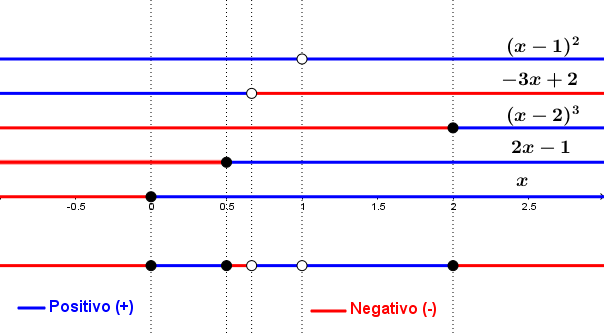
\includegraphics[width = 320px]{Q1b.png}
 \end{center}


\item {\bf (1,0)} $\ds \frac{1}{|2x+1|}\leq  \frac{1}{1-x}$\\
Primeiro reformulamos a inequação:
 $$\frac{1}{|2x+1|} - \frac{1}{1-x} \leq 0$$
 $$\frac{1-x - |2x+1|}{|2x+1|(1-x)} \leq 0$$
Usando a definição do módulo: $ 1-x - |2x+1| =  \left\{
\begin{array}{ll}
      x+2 & \mbox{se }  x < -\frac{1}{2} \\
      -3x & \mbox{se } x \geq -\frac{1}{2} \\
\end{array} 
 \right.$ Daí que esta expressão é positiva se, e somente se, $-2 \leq x \leq 0$. Então podemos fazer o estudo do sinal\\
 \begin{center}
 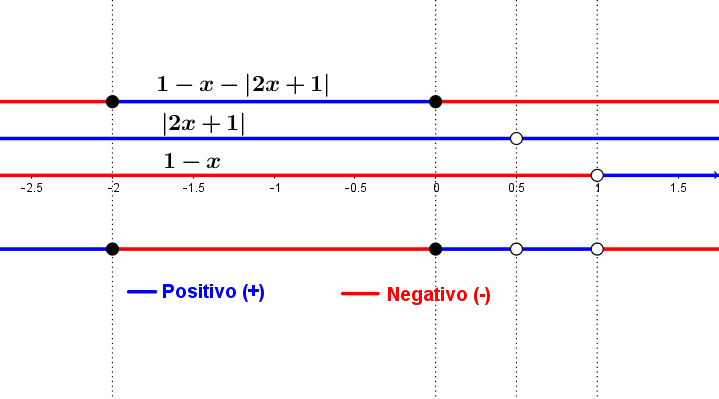
\includegraphics[width = 320px]{Q1c.png}
 \end{center}
 e concluir que o conjunto-solução é $\left[2, -\frac{1}{2}\right) \cup \left(-\frac{1}{2}, 0\right] \cup \left(1, +\infty\right)$.
\end{enumerate}	
\vspace{5mm}
\item	
	\begin{enumerate}
	\item {\bf (1,0)} Mostre que $\ds\frac{\sqrt{2}}{\sqrt{5}}+1$ não é racional.\\ 
	\vspace{3mm}
	Suponhamos que $\frac{\sqrt{2}}{\sqrt{5}}+1$ seja racional.\\
 Sabemos que $1\in\mathbb{Q}$ e que a subtração de racionais é racional, logo devemos ter $\frac{\sqrt{2}}{\sqrt{5}}\in\mathbb{Q}$.\\
 Se $\frac{\sqrt{2}}{\sqrt{5}}\in\mathbb{Q}$ então $\exists p,q\in\mathbb{Z}$ onde $p$ e $q$ não tem fatores em comum e $\frac{p}{q}=\frac{\sqrt{2}}{\sqrt{5}}$.\\
 Daí temos que $\frac{p^2}{q^2}=\frac{2}{5}\Rightarrow5p^2=2q^2$.\\
 Vemos que $5p^2$ é par e como $2$ não divide $5$ temos que $p^2$ é par e consequentemente $p$ é par, pois todo quadrado de um número par é sempre par.\\
 Seja então $p=2r$, temos que $5.(2r)^2=2q^2\Rightarrow5.2r^2=q^2$.\\
 Daí vemos que $q^2$ é par e consequentemente $q$ é par, o que é um absurso pois $p$ e $q$ não tem fatores em comum.\\
 Logo $\frac{\sqrt{2}}{\sqrt{5}}\not\in\mathbb{Q}$ e consequentemente $\frac{\sqrt{2}}{\sqrt{5}}+1$ não é racional.
	\item {\bf (1,0)} Esboce uma figura que represente um segmento de reta de medida $\sqrt{7}$. (Construir a partir da unidade como em aula).\\
	São muitas soluções possíveis, mas entre elas:
	\begin{center}
	  
\includegraphics[width = 320px]{Q2b.png}
	\end{center}
	\end{enumerate}
	
\vspace{5mm}

\item Seja $f(x)=|x-1|+|x-2|$.
\begin{enumerate}
\item {\bf (0,5)} Dê o domínio de $f$.\\
 %TODO ver como deixar só um parêntese e como deixar em negrito
 Como os módulos estão definidos para todos os reais $\mathrm{Dom}(f) = \RR$.

\item {\bf (0,5)} Escreva uma expressão para $f$ sem usar o valor absoluto. (Sugestão: dividir o domínio em intervalos apropriados).\\
 \begin{itemize}
  \item se $x<1$ temos\\
  $f(x)=-(x-1)-(x-2)$\\
  $f(x)=-2x+3$\\
  \item se $1\leq x<2$ temos\\
  $f(x)=+(x-1)-(x-2)$\\
  $f(x)=1$
  \item se $x\geq2$ temos\\
  $f(x)=+(x-1)+(x-2)$\\
  $f(x)=2x-3$\\
  \end{itemize}
 Logo, $ f(x) =  \left\{
\begin{array}{ll}
      -2x+3 & \mbox{se }  x < 1 \\
      1 & \mbox{se } 1 \leq x < 2\\
      2x-3 & \mbox{se } 2 \leq x
\end{array} 
 \right. $\\

\item  {\bf (0,5)} Esboce o gráfico de $f$.
\begin{center}
 
\includegraphics[width = 320px]{Q3c.png}
\end{center}
\end{enumerate}

\vspace{5mm}
\item Responda Verdadeiro ou Falso nas sentenças abaixo, justificando suas respostas.
\begin{enumerate}

\item{\bf (0,5)} Sejam $x,y\in \RR$ então $x<y$ se, somente se $x^2<y^2$.\\
 Falso. Considere $x=-2$ e $y=-1$. Temos $x<y$; mas $x^2 = 4 > 1 = y^2$.
\vspace{3mm}
\item{\bf (0,5)} Sejam $x,y\in \RR$ então $x<y$ se, somente se $x^3<y^3$.\\
Verdadeiro.
Vamos supor $x < y$ e analisar os casos possíveis:

 \begin{description}
 \item[1º Caso:] $x$ e $y$ têm o mesmo sinal.\\
 Primeiro parafraseamos a conclusão para facilitar a análise.\\
 $$x^3 < y^3$$
 $$x^3 - y^3 <0$$
 $$(x-y)(x^2+xy+y^2) < 0$$
 Sabemos por hipótese que $x-y < 0$. Basta então mostrar que $x^2+xy+y^2$ é um número positivo. Já sabemos de cara que $x^2, \ \ y^2 > 0$; pois $x, \ \ y \neq 0$. O $xy$ também é positivo, pois $x$ e $y$ têm o mesmo sinal. Daí que a soma $x^2+xy+y^2$ de números positivos certamente será também positiva. 
  
 \item[2º Caso:] $x$ e $y$ têm sinais diferentes, incluindo a possibilidade de um ser zero.\\
 O cubo de um número negativo/nulo/positivo continua sendo negativo/nulo/positivo. Daí que a ordem não se altera nesse caso.
 \end{description}
 Isso prova que $x<y \Rightarrow x^3 < y^3$; mas será que $x^3 < y^3 \Rightarrow x < y$? Basta tomar a contrapositiva $x \geq y \Rightarrow x^3 \geq y^3$ e aplicar o mesmo raciocínio.
\vspace{3mm}
\item{\bf (0,5)} Se $x\geq 0$ então $x\geq \sqrt{x}$.\\
Falso. Seja $x=\frac{1}{4}$. Temos que e $\frac{1}{4} < \sqrt{\frac{1}{4}} = \frac{1}{2}$.
\end{enumerate}

\vspace{5mm}
\item Considere a chamada "regra 95" para a previdência.  Nesta regra o trabalhador teria direito à aposentadoria quando a soma de sua idade com o número de anos de serviço atingisse $95$. 

\begin{enumerate}
\item {\bf (0,5)} Baseado na regra $95$ quem começou a trabalhar aos $25$ anos teria direito à aposentadoria com que idade?\\
\vspace{3mm}
Se $x$ é a idade da pessoa temos que $x+(x-25)=95\Rightarrow x=60$. Portanto a pessoa tem direito de se aposentar aos $60$ anos.
\item {\bf (1,0)} Sendo $x$ a idade com que uma pessoa começa a trabalhar, encontre a idade com que ele tem direito à aposentadoria $f(x)$.\\
\vspace{3mm}
Seja $x$ a idade que a pessoa começa a trabalhar e $f(x)$ a idade que a pessoa tem o direito de se aposentar. Sabemos que a soma da idade que a pessoa tem o direito de se aposentar com o tempo de serviço deve ser igual a 95.
 Sabemos que o tempo se serviço é dado pela idade da pessoa menos a idade que ela começou a trabalhar, então $f(x)+(f(x)-x)=95\Rightarrow f(x)=\frac{1}{2}(95+x).$
\item{\bf (0,5)}  Esboce o gráfico de $f$, considerando que a idade é um número real não negativo e que é proibido trabalhar antes dos $16$ anos.
\begin{center}
 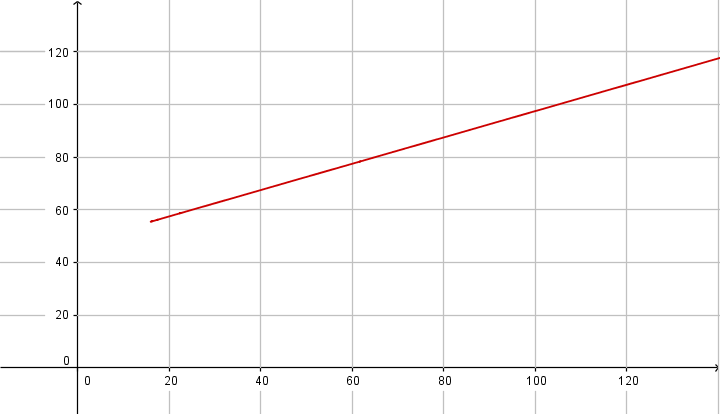
\includegraphics[width = 320px]{Q5c.png}
\end{center}
\end{enumerate}
\end{enumerate}
\end{document}
